\documentclass[11pt]{article}
\usepackage{graphicx} % Required for inserting images
\usepackage{hyperref}
\usepackage{listings}
\usepackage{caption}
\usepackage{minted}
\usepackage{todonotes}
\usepackage[a4paper, total={6in, 8in},margin=1in,top=0.81in,bottom=1.25in]{geometry}
\usepackage{fancyhdr}
\usepackage{pdfpages}
\usepackage{sectsty}
\usepackage{fontspec}
\usepackage{multicol}

\setmainfont{Carlito}
\sectionfont{\fontsize{24}{30}\selectfont}  % 24pt size, 30pt line spacing
\subsectionfont{\fontsize{18}{24}\selectfont}
\subsubsectionfont{\fontsize{14}{18}\selectfont}
\renewcommand{\listingscaption}{Izvorni kod}
\renewcommand{\listoflistingscaption}{Spisak izvornih kodova}
\pagestyle{fancy}
\fancyhf{}
\fancyfoot[L]{\fontsize{11}{13}\selectfont Aleksa Bajat, Intermedijarne reprezentacije izvornog koda u prednjem kraju (frontend-u) rustc kompajlera}
\fancyfoot[R]{\newline\fontsize{11}{13}\selectfont \thepage}

\title{Intermedijarne reprezentacije izvornog koda u prednjem kraju (frontend-u) rustc kompajlera}
\author{Aleksa Bajat}
\date{September 2024}

\begin{document}


\includepdf[pages={1-6}]{MscTemplate.pdf}
\section{Spisak skraćenica}
\tableofcontents
\section{Uvod}

U svetu razvoja sistema visokih performansi, operativnih sistema, drajvera i bilo kog drugog kritičnog softvera koriste se jezici niskog nivoa kao što su C i C++.
Tokom godina Microsoft je uvideo da je preko 70\% bezbednosnih slabosti nastalo pogrešnom manipulacijom i korupcijom memorije [1]. 
C nema odbrambene mehanizme od ovakvih problema (pored potencijalnih dodatnih upozorenja koja se mogu ostvariti dvostrukom upotrebom GCC i Clang kompajlera), dok C++ uprkos dodavanju konstrukta kao što su \verb|unique_ptr|, \verb|shared_ptr| i \verb|weak_ptr| interoperabilnost sa starijim standardima ili bibliotekama zahteva korišćenje sirovih pokazivača. 

Rust jezik je nastao sa ciljem da reši ovaj problem. Podrazumevana upotreba jezika je inherentno bezbedna sa aspekta memorije i paralelizma. Bezbednost se ostvaruje robustnim sistemom tipova, novog načina rukovanja memorijom i veoma striktnog \verb|rustc| kompajlera.
U C++ ekosistemu koriste se softverski obrasci kao što je \verb|Scope-bound Resource Management| da bi se standardizovala alokacija i dealkoacija memorije, ali korisnik jezika nije primoran da softvrski obrazac upotrebi. U Rust jeziku izbor ne postoji, na kraju svakog opsega vrši se automatska dealokacija memorije preko \verb|borrow checker| mehanizma (nije potreban manuelni poziv \verb|free|).
C i C++ poseduju veoma dvosmislene i neprecizne poruke kada se greška dogodi dok Rust jezik karakterišu veoma precizne poruke koje opisuju gde se desila greška i kako je potencijalno rešiti.

Prvobitna verzija Rust kompajlera je napisana u \verb|O'Caml| jeziku, dok je svaka sledeća verzija napisana u samom Rust-u.
Medjutim treba imati na umu da je Rust samo \verb|frontend| nad \verb|LLVM|-om. LLVM je kolekcija modularnih i ponovo iskoristivih tehnologija za izradu kompajlera. Rust se oslanja u potpunosti na \verb|LLVM| prilikom generisanja mašinskog koda, dok je svaki drugi deo
(\verb|frontend|) napisan potpuno ispočetka.
Veliki deo Rust jezika je izuzetno inovativan i samim tim to je razlog da se detaljno istraži kako u pozadini funkcioniše.

Reprezentacija izvornog koda jeste prikaz ili skup prikaza izvornog koda korisnika jezika koji obezbedjuju tipove, dijagnostiku,
automatsku dealokaciju memorije i ostale ergonomske i funkcionalne delove jezika.
\newpage

\section{Pozadina}

U ovoj sekciji obradjuje se pozadina iza \verb|Rust| jezika, zvaničnog menadžera paketa \verb|Cargo| i 
LLVM seta alata.

\subsection{Rust jezik}

\verb|Rust| je statički tipiziran jezik koji je nastao 2006. godine kao lični projekat \verb|Graydon| \verb|Hoare|-a, radnika kompanije 
Mozila. Uvidevši potencijal jezika, Mozila je započela sponzorisanje projekta 2010. godine kada je jezik i javno 
predstavljen \cite{rust-language}. \verb|Rust| je jezik niskog nivoa koji se fokusira na memorijsku bezbednost
i bezbedan paralelizam bez oslanjanja na skupljač smeća (\verb|garbage| \verb|collector|). Skupljač smeća 
obično uvodi lakoću programiranja na uštrb nedeterminističkih performansi usled oslobadjanja memorije 
sa \verb|heap|-a, na memorijskim lokacijama gde je brojač referenci na nuli. U jezicima bez skupljača 
smeća obično postoji odredba koja se poziva da bi se dinamički alocirana memorija oslobodila. \verb|Rust|
jezik uvodi sasvim novi koncept u domen programskih jezika, pozajmljivač (\verb|borrow| \verb|checker|).
Pozajmljivač se zasniva na striktnoj primeni menadžmenta resursa u opsegu (\verb|scope-bound| \verb|resource| \verb|management|) 
od strane kompajlera. Ovo je softverski obrazac koji je preporučljivo koristiti u nebezbednim jezicima 
niskog nivoa. Naime u prirodi softverskog obrasca jeste da ga nije moguće primorati, osim ako nije direktno
integrisan u jezik kao što je slučaj sa jezikom \verb|Rust|. Ključan koncept koji se uvodi uz pozajmljivač 
jeste vlasništvo. Vlasništvo predstavlja dužnost da opseg koji direktno manipuliše memorijom (pristup memoriji nije 
pridobijen referencom) tu memoriju na kraju opsega oslobodi. 

U jeziku \verb|C| postoje dva načina deljenja 
memorije: preko vrednosti i preko reference (pokazivača). Deljenje preko vrednosti (kopija) je
podrazumevano. U \verb|Rust|-u ne postoji deljenje preko vrednosti, već je osnovna akcija prenos vlasništva.
Deljenje preko vrednosti se može simulirati kloniranjem (funkcija \verb|clone|) koju prati prenos vlasništva.
Opseg u kome je memorija dodeljena varijabli validna 
se naziva životni vek. Vlasništvo onemogućuje brojne greške kao što su korišćenje nakon oslobadjanja i curenje 
memorije tj. aktivno vrši zabranu nedefinisanih stanja. Program se ne kompajlira uspešno ukoliko pravila 
vlasništva nisu zadovoljena. Izvorni kod \ref{lst:use_after_free_c} predstavlja C kod koji koristi memoriju 
nakon oslobadjanja. Uspešno se kompajlira ali prilikom izvršavanja vraća grešku. Sa druge strane u izvornom 
kodu \ref{lst:user_after_free_rust} predstavljen je isti koncept u \verb|Rust| jeziku. Funkcija 
\verb|drop| preuzmima vlasništvo nad memorijom 
i oslobadja je, simulirajući kraj opsega. Izvorni kod \ref{lst:user_after_free_rust} se neće 
uspešno kompajlirati jer se vrši pokušaj manipulacijom memorije nad varijablom kojoj je prošao životni vek.
Ujedno je demonstrirano da korisnik \verb|Rust| jezika ne mora da brine o životnom veku varijable, isključujući
curenje memorije kao opcije.

\begin{multicols}{2}
    \begin{listing}[H]
    \begin{minted}{C}
int* pointer = malloc(sizeof(int));
*pointer = 5;
pointer = NULL;
free(pointer);
*pointer = 6; 
    \end{minted}
    \caption{Korišćenje nakon oslobadjanja - C}
    \label{lst:use_after_free_c}
    \end{listing}
    \columnbreak
    \begin{listing}[H]
    \begin{minted}{rust}
let mut a: Box<i32> = Box::new(5);
drop(a);
*a = 6;
    \end{minted}
    \caption{Korišćenje nakon oslobadjanja - Rust}
    \label{lst:user_after_free_rust}
    \end{listing}
\end{multicols}

U jeziku \verb|C++|, dobra praksa je pravilno označavati nepromenljivost reference ili vrednosti
unutar funkcija korišćenjem ključne reči \verb|const|, obaveštavajući budućeg korisnika funkcije 
o promenljivosti. U jeziku \verb|Rust|, promenljivost mora da se naznači ekspicitno upotrebom ključne 
reči \verb|mut|. Inverzija principa je omogućila daleko bolju čitljivost i razumevanje koda.

Bezbedni paralelizam je jedna od glavnih odlika \verb|Rust| jezika. Realizuje se pomoću osobina (\verb|trait|)
i vlasništva. Osobine su ugovor koji se postavlja nad strukturom i po funkcionalnosti liče na interfejse
u drugim jezicima. Glavna razlika je u fleksibilnosti. Osobine mogu da se implementiraju nad tipovima
koje nismo mi definisali, na primer iz drugih biblioteka. Razlog tome jeste baš u ključnoj reči ugovor.
Ako struktura zadovoljava ugovor koji osobina nalaže (obično ispunjenje drugih osobina ili
metoda) onda je osobina primenljiva nad strukturom. Ključne osobine koje realizuju bezbednost podataka
u paralelnom okruženju jesu \verb|Sync| i \verb|Send|. Tip je \verb|Send| ako je bezbedno poslati ga 
u drugu nit. Tip je \verb|Sync| ako ga je bezbedno deliti izmedju niti. Tipovi sačinjeni od drugih tipova koji
implementiraju \verb|Sync| i/ili \verb|Send| su automatski \verb|Sync| i/ili \verb|Sync|. Skoro sve primitive
unutar \verb|Rust| jezika su \verb|Send| i \verb|Sync|. U bitnije izuzetke spadaju sirovi pokazivači jer nemaju
bezbednosne garancije, \verb|UnsafeCell| (samim tima i \verb|Cell| i \verb|RefCell|) jer implementiraju
unutrašnju mutabilnost čime je tip rizik u vidu štetnog preplitanja, kao i \verb|Rc| (brojač referenci) 
jer je broj referenci deljen i nesinhronizovan. Uz \verb|std::marker|, ove osobine su jedine primitive koje su 
deo samog kompajlera, a ne standardne biblioteke.

Atributi su zaglavlja koja pružaju dodatne informacije kompajleru. Atributi mogu biti spoljašnji ili 
unutrašnji \ref{lst:attributes}. Primenjuju se na brojne konstrukte unutar jezika kao što su eksterni blokovi,
funkcije, moduli i enumeracije. Atributi generišu kod, isključuju ili uključuju dijagnostiku, 
postavljaju limitacije i udeluju u testiranju. 

\begin{listing}[H]
\begin{minted}{rust}
// Spoljašnji atribut se primenjuje na tip koji sledi 
// nakon atributa koji pri tome nije atribut.
#[allow(dead_code)] 
fn main() {
    // Unutrašnji atribut.
    // Primenjuje se na vlasnika lokalnog opsega. 
    #![allow(unused_variables)]
    let x = 10;  
}
\end{minted}
\caption{Spoljašnji i unutrašnji atributi}
\label{lst:attributes}
\end{listing}

Makro sistem je jedan od najmoćnijih delova \verb|Rust| jezika. Makroi su kod koji generiše drugi kod i ovaj 
način programiranja se naziva metaprogramiranje. 
Korisni su da bi se smanjila količina koda koja mora da se održava, ali i da bi se izbeglo višestruko pisanje 
veoma sličnog koda (\verb|boilerplate|). Postoji četiri vrste makroa: deklarativni, funkcijski, proceduralni i atributski. 
Deklarativni i funkcijski su slični po prirodi, pozivaju se nalik običnim funkcijama ali u imenovanju imaju sufiks "!".
Deklarativni makroi moraju deterministički navesti broj parametara, dok funkcijski imaju proizvoljan broj parametara.
Jedan od najčešće korišćenih deklarativnih makroa jeste \verb|vec!| koji služi da smanji broj linija koda da bi se 
inicijalizovao vektor. Sa druge strane funkcijski makroi mogu da se koriste da bi se pisala sintaksa nekog drugog jezika, 
što je i česta pojava u \verb|Rust| bibliotekama koje pozivaju \verb|SQL| ili \verb|Python|.
Proceduralni makroi su makroi koji uvoze kroz predefinisani \verb|derive| atribut, dok atributski makroi generišu sasvim 
novi atribut. Glavna razlika izmedju njih jeste u fleksibilnosti. Proceduralni makroi rade na strukturama i enumeracijama,
dok atributski makroi mogu biti definisani da rade i nad drugim stavkama jezika poput funkcija.

\verb|Rust| jezik se odlikuje apstrakcijama bez cene. Osobina apstrakcija bez cene označava da koncepti 
višeg nivoa kao što su kolekcije i generički tipovi ne utiču na performanse programa prilikom njegovog izvršavanja.
\verb|Rust| omogućava ovu karakteristiku putem monomorfizacije. Monomorfizacija je proces putem kojeg se kreira 
kopija generičkog koda za svaki konkretan tip koji koristi generički kod tj. generički kod se pretvara u 
negenerički kod. Naime ovaj proces povećava veličinu krajnjeg izvršnog fajla i produžava vreme kompajliranja.
Generičke strukture mogu da imaju najveći uticaj na veličinu izvršnog fajla. Problem se amortizuje 
tako što se ne generišu metode za konkretan tip ako ih isti ne koristi u izvornom kodu.


\newpage
\subsection{Cargo}

U Rustu, \verb|Crate| je najmanja jedinica organizacije koda. Postoje dva osnovna tipa, izvršni programi i biblioteke.
Izvršni programi sadrže \verb|main| funkciju i mogu da se izvršavaju. Biblioteke se ne izvršavaju i nemaju potrebu za \verb|main|
funkcijom već pružaju funkcionalnosti koje se mogu koristiti u drugim \verb|Crate|-ovima. 

Skoro svaki modreni jezik dolazi sa jednim ili više menadžera paketa (biblioteka). Zvanični menadžer paketa u \verb|Rust|
ekosistemu se naziva \verb|Cargo|. Glavni zadatak mu je da beleži zavisnosti programa tako da je moguće rekreirati 
program na deterministički način. Uvode se \verb|Cargo.lock| i \verb|Cargo.toml|
fajlovi. \verb|Cargo.toml| je manifest fajl koji održava korisnik. Sastoji se meta podataka poput naziva i verzija kao i spiska paketa sa korisnički definisanim 
verzijama (ili opsegom verzija) koji se trenutno koriste u programu. Pored verzije, paketi mogu da imaju funkcionalnosti koje korisnik mora eksplicitno da navede ukoliko su potrebni.
\verb|Cargo.lock| se generiše nakon koraka kompajliranja ali ga je moguće izgenerisati kroz \verb|cargo| \verb|generate-lock| komandu.
\verb|Cargo.lock| omogućava da se pri kompajliranju programa na potenicjalno različitim mašinama koriste identični paketi praćenjem tačne verzije svakog pojedinačnog paketa.

\verb|Cargo| dobavlja zavisnosti iz registra. Registar sadrži indeks u kome se nalazi lista dostupnih \verb|Crate|-ova. Podrazumevani javni registar je \verb|crates.io|, ali je moguće 
konfigurisati sopstveni registar koji je proizvoljne vidljivosti. Jedan \verb|Crate| može koristiti zavisnosti iz različitih registara. Ukoliko se \verb|Crate| nalazi u registru koji nije 
podrazumevani u \verb|Cargo.toml| fajlu se za tu zavisnost definiše \verb|registry| atribut.

\verb|Cargo| je otporniji od menadžera paketa iz drugih ekosistema jer nije moguće brisati verzije jednom kada je paket objavljen na javnom registru. 
Ovaj pristup sprečava napade lanca snabdevanja kao što se desilo u \verb|JavaScript| menadžeru paketa \verb|NPM|. Paket \verb|left-pad| 
je sačinjen od 11 linija koda koji dodaje specificiranu količinu razmaka sa leve strane niza karaktera. Iako je paket trivijalan, mnoge biblioteke koje 
su masivno korišćene su direktno ili indirektno zavisile od njega. Problem je nastao kada je kreator \verb|left-pad| paketa obrisao 
paket sa repozitorijuma poremetivši ogroman deo ekosistema. U softveru otvorenog koda napadi lanca snabdevanja postaju sve češći (preko 700\% povišena učestalost
iz godine u godinu) i zbog toga regulatorne uprave rade na standardizaciji menadžera paketa ne bi li se ovakvi napadi sprečili \cite{supply-chain}.

Nekada je \verb|Crate|-u neophodno da kompajlira ili \verb|link|-uje neki kod koji nije napisan u Rust-u, na primer C kod. Koristeći poseban fajl \verb|build.rs| u korenskom direktorijumu 
projekta moguće je definisati skriptu koju će \verb|rustc| da kompajlira i izvrši pre kompajliranja ciljanog \verb|Crate|-a. Podrazumevano je da se skripta izvršava pred svaku kompilaciju,
ali je moguće definisati putanju ili promenljivu okruženja prilikom čije promene će se skripta ponovo (sledeći put kada se kompajlira \verb|Crate|) izvršavati.

\verb|Cargo| pored distribuiranja paketa pruža razne olakšice i automatizacije u odnosu na sirovo korišćenje \verb|Rust| kompajlera. 
Komanda \verb|cargo init| se koristi da bi se jednostavno inicijalizovao novi \verb|Crate| zajedno sa \verb|Cargo.toml| fajlom. 
Komande \verb|cargo| \verb|add| i \verb|cargo| \verb|remove| dodaju i brišu paket iz \verb|Cargo.toml| fajla.
Komanda \verb|cargo| \verb|check| kompajlira trenutni \verb|Crate| bez generacije koda (bez upotrebe LLVM-a) što je značajno brže 
od pokretanja \verb|cargo| \verb|build| koji i generiše kod. Ovo je korisno jer je većinski deo dijagnostike zasnovan 
na koracima pre generisanja koda. Komanda \verb|cargo| \verb|run| konstriše paket i izvršava ga. Ovo je značajno jer u većini slučajeva korisnik želi da pokrene program nakon što je 
napisao izmenu i izbegava \verb|CLI| gimnastiku dolaska do \verb|/target| foldera i pokretanja izvršnog fajla. 
Komanda \verb|cargo| \verb|test| pokreće sve \verb|unit| testove koji se definišu upotrebom atributa \verb|test| nad funkcijama.
Budući da je \verb|Cargo| delom apstrakcija nad \verb|rustc| kompajlerom i da je \verb|rustc| izuzetno konfigurabilan, koristi se komanda \verb|cargo| \verb|rustc|
koja prima dodatne kompajlerske opcije.

\newpage

\subsection{LLVM projekat}

Generisanje koda je jedan od najtežih zadataka prilikom kreiranja novog kompajlera. Izvorni kod koji 
korisnici pišu se prevodi u mašinski kod i pre svega mora biti tačan. Pored tačnosti cilj prilikom 
dizajniranja generatora koda jeste laka implementacija, testiranje i održavanje.
Prilikom prevodjenja obično postoji 
više medju reprezentacija izvornog koda sa ciljem da validira i optimizuje izvorni kod. Medju reprezentacije 
se svrstavaju u \verb|frontend| ili u \verb|backend|. \verb|Frontend| ima za zadatak da skenira, parsira 
i prevede izvorni kod u relativno nisku medju reprezentaciju. \verb|Backend| stoga može da pretpostavi 
da su sve statičke sintaktičke i semantičke greške detektovane i da su tipovi i njihove konverzije
obradjene na osnovu čega optimizuje i generiše kod za ciljanu arhitekturu.

LLVM projekat je skup modularnih i ponovo iskoristivih kompajlerskih tehnologija \cite{llvm}. Pod okriljem \verb|LLVM|-a
se nalaze brojni projekti. Glavni projekat je \verb|LLVM| \verb|Core| unutar koga je specificirana \verb|LLVM|
medju reprezentacija (\verb|LLVM| \verb|IR|) na kojoj se zasniva modularnost. Nad \verb|LLVM| medju reprezentacijom
je implementiran optmizator čiji kod se prosledjuje generatoru (\verb|backend|-u) koda cljane arhitekture. Samim time 
bilo koji \verb|frontend| koji se napiše tako da je krajnji izlaz \verb|LLVM| \verb|IR| može da iskoristi 
ostale delove kompajlera bez ikakvih dodatnih izmena \ref{lst:llvm_modular}.

\begin{listing}[H]
\begin{center}
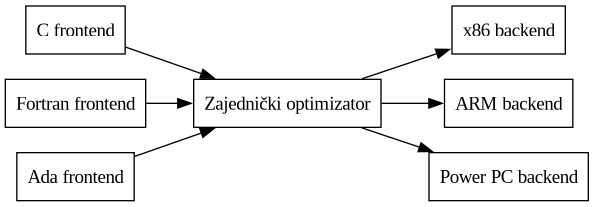
\includegraphics[width=5in, height=1.6in]{assets/images/modern_compiler_design.png}
\end{center}
\caption{Modularnost LLVM-a}
\label{lst:llvm_modular}
\end{listing}

Postoje brojne vrste optimizacije koje se mogu izvršiti nad izvornim kodom. Optimizacije se obično svode 
na tri osnovna koraka, pronalazak šablona koji se treba transformisati, validirati da li je bezbedno primeniti 
transformaciju i izvršavanje transformacije \cite{oss-architecture}. Optimizacije u \verb|LLVM| optmizatoru su modularne i izvršavaju 
se nad \verb|LLVM| medju reprezentacijom. Svaka \verb|LLVM| optmizacija je napisana kao \verb|C++| klasa koja 
nasledjuje \verb|Pass| (prolazak) klasu. Većina prolazaka je napisana u jedanom \verb|.cpp| fajlu.
Stoga otvara se mogućnost da se dodaju optimizacije specifične za jezik. Svaki prolazak se kompajlira u jedan 
ili više relokatabilnih objekata, (\verb|.o|) fajlova koji se potom grupišu u arhivne (\verb|.a|) fajlove. Objektni fajlovi 
su mašinski kod pre procesa linkovanja. Linkovanje je proces skupljanja i kombinovanja relokatabilnih objektnih fajlova
u jedan izvršni objektni fajl. Prilikom linkovanja nekog \verb|.o| fajla sa \verb|.a| fajlom linker će 
za svaki do tada nespojen simbol probati da nadje vezu u svim \verb|.o| fajlovima arhive.

\verb|LLVM| generator koda je odgovaran za prevodjenje \verb|LLVM| medju reprezentacije u mašinski kod ciljane 
arhitekture. Idealno za svaku arhitekturu postojao bi specifičan kod za prevodjenje, ali u isto vreme 
svi generatori rade vrlo sličan posao. Slično kao i kod optimizacije proces generisanja koda se deli u prolaske,
izbor seta instrukcija, način alokacije registara, planiranje (\verb|scheduling|), optimizacija rasporeda 
koda i generisanje asemblerskog koda. Pri kreiranju generatora za novu ciljnu arhitekturu svaki od ovih prolazaka
može ponovo da se iskoristi, modifikuje ili potpuno zameni.

\verb|LLVM| medju reprezentacija se veoma efikasno serijalizuje u i deserializuje iz \verb|LLVM| bitkoda. 
Ova efikasnost otvara mogućnost za optimizaciju u vreme linkovanja \ref{lst:link_time_opt}. To je još jedan set optimizacionih prolazaka 
koji dodatno poboljšava kranji mašinski kod. Linker prepoznaje da se u \verb|.o| fajlovima nalazi 
\verb|LLVM| bitkod umesto mašinskog koda, učitava ih u memoriju, linkuje ih, a potom izvršava \verb|LLVM|
optimizator nad mnogo većom celinom koda, omogućavajući daleko agresivnije optimizacije. 
Ova opcija se uključuje dodavanjem \verb|-O4| opcije komandne linije. 

\begin{listing}[H]
\begin{center}
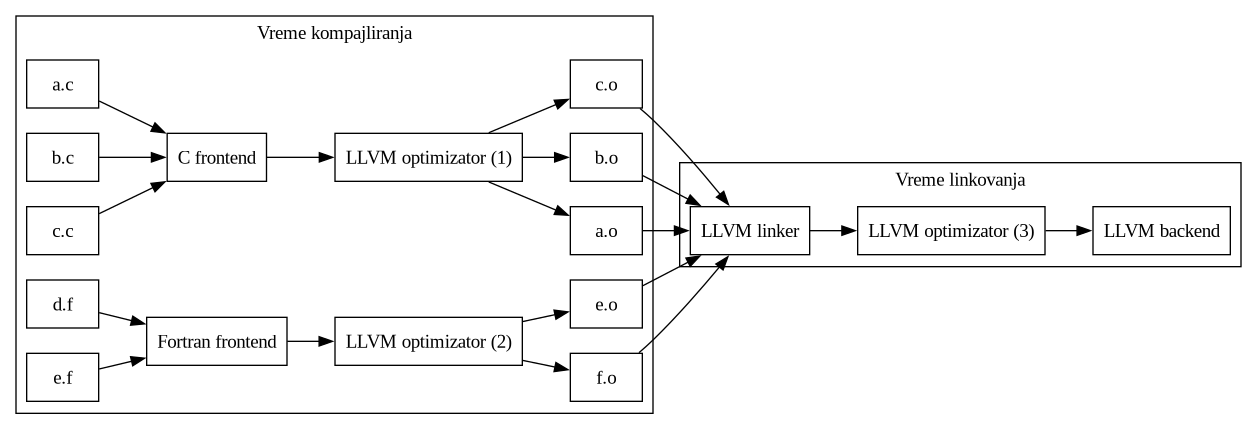
\includegraphics[width=6in, height=2.2in]{assets/images/link_time_optimization.png}
\end{center}
\caption{Optimizacija u vreme linkovanja}
\label{lst:link_time_opt}
\end{listing}

\verb|LLVM| medju reprezentacija podesća na asemblerski jezik. Strogo je tipiziran i poseduje jednostavne 
tipove poput celih brojeva, brojeva sa pokretnim zarezom, pokazivača i struktura. Jedna od glavnih razlika 
u odnosu na asembler jeste to što ne koristi ograničeni broj imenovanih registara već koristi beskonačan 
skup promenljivih koje se definišu sa \verb|%| prefiksom. Neki detalji mašine su apstrahovani od korisnika 
poput poziva funkcija (\verb|call|) i vraćanja vrednosti (\verb|ret|) \ref{lst:llvm_ir}.

\begin{listing}[H]
\begin{minted}{llvm}
define i32 @add2(i32 %a, i32 %b) {
entry:
  %tmp1 = icmp eq i32 %a, 0
  br i1 %tmp1, label %done, label %recurse

recurse:
  %tmp2 = sub i32 %a, 1
  %tmp3 = add i32 %b, 1
  %tmp4 = call i32 @add2(i32 %tmp2, i32 %tmp3)
  ret i32 %tmp4

done:
  ret i32 %b
}
\end{minted}
\caption{LLVM medju reprezentacija}
\label{lst:llvm_ir}
\end{listing}

\verb|Rust| jezik je \verb|frontend| nad \verb|LLVM|-om. Postoji puno olakšica u ovom pristupu.
\verb|Rust| tim ima cilj da izgeneriše pravilnu \verb|LLVM| medju reprezentaciju, na osnovu koje 
\verb|LLVM| izvršava optimizacione prolaske i generiše kod. Greške prilikom generisanja koda ne mora da 
održava \verb|Rust| tim, što značajno smanjuje količinu ljudi koja aktivno mora da bude uključena u razvoj. 
Svaka distribucija koju \verb|LLVM| podržava automatski podržava i \verb|Rust|. Optimizacije se ne moraju 
posebno pisati i održavati jer \verb|LLVM| već poseduje značajan broj čestih optimizacija. \verb|Rust| 
omogućava kompajliranje na osnovu više \verb|LLVM| verzija, poslednja glavna verzija je uvek podržana,
i obično su podržane jedna ili dve ispod nje.

\section{Rust kompajler}

Rust kompajler u svakom trenutku poseduje tri glavne verzije skupa alata (\verb|toolchain|): stabilna, beta i noćna (\verb|nightly|) verzija.
Stabilna verzija kompajlera je bezbedna i preporučena za produkcionu upotrebu. Beta verzija sadrži funkcionalnosti
koje se usvajaju u narednoj stabilnoj verziji. Noćna verzija je verzija kompajlera koja se 
proizvodi svaku noć, sa svim najnovijim netestiranim promenama. Kapija funkcionalnosti je mehanizam bezbednosti
koji onemogućava da eksperimentalne (nestabilne) funkcionalnosti slučajno završe u produkciji. 
Kapija je definisana na osnovu stanja kapije, naziva funkcionalnosti, verzije, broja zahteva za povlačenjem
(\verb|pull| \verb|request|) i opcionog komentara.
Stanje kapije funkcionalnosti može biti nestabilno, obrisano ili prihvaćeno i nekompletirano. Nekompletirano 
stanje unutar kapije daje do znanja korisniku noćne verzije ili drugim saradnicima da je nestabilna funkcionalnost 
u razvoju.  Nestabilne kapije onemogućavaju da stabilna i beta verzija kompajlera kompajliraju 
dati segment koda (ignoriše se).  Samim time razvoj je direktno 
usmeren ka noćnoj verziji koja je pod nadzorom celokupnog Rust tima. Obrisane kapije se ne brišu fizički iz koda,
već se status kapije promeni u obrisan uz komentar sa razlogom. Na ovaj način se čuva istorija pokušanih 
funkcionalnosti sa razlozima koji su uzrokovali brisanje. U slučaju da se sličan zahtev ponovo javi, retrospektiva
služi kao moćan alat koji će idealno upozoriti saradnike i preusmeravati ih na bolji pravac.

\begin{listing}[H]
\begin{minted}{rust}
    (incomplete, pub_restricted, "CURRENT_RUSTC_VERSION", Some(32409)),
    (unstable, pub_restricted, "CURRENT_RUSTC_VERSION", Some(32409))
    (accepted, pub_restricted, "CURRENT_RUSTC_VERSION", Some(32409)),
    (removed, pub_restricted, "CURRENT_RUSTC_VERSION", 
    Some(32409), Some("Removed because.."))
\end{minted}
\caption{Kapija funkcionalnosti}
\label{lst:rustup_set}
\end{listing}

Svaka funkcionalnost prolazi kroz dugačak proces provera pre nego 
što se usvoji. Ukoliko funkcionalnost zahteva promene koje nisu reorganizacija, refaktorisanje, dokumentovanje
i slično, kreira se zahtev za komentare (\verb|RFC|) koji detaljno objašnjava važnost funkcionalnosti i 
pregled implementacionih detalja sa visine. U suprotnom ovaj segment se preskače. Stejkholderi kao što je Rust kompajler tim, ali i sama Rust zajednica 
ima pravo da vaga o potencijalnim implikacijama koje funkcionalnost donosi. Odobravanje zahteva znači početak 
razvoja ali ne garantuje usvajanje. Ukoliko je funkcionalnost razvijena, pokrivena testovima, 
bez značajnih primedbi, bilo koji saradnik može pokrenuti zahtev za stabilizaciju. Zahtev je konstituiran iz 
četiri dela: dokumentacionog \verb|pull| \verb|request|-a, stabilizacionog izveštaja, 
perioda finalnog komentara i stabilizacionog \verb|pull| \verb|request|-a.

Dokumentacija funkcionalnosti koja se stabilizuje se briše iz nestabilne knjige \cite{unstable} i ažurira se 
dokumentacija namenjena korisnicima jezika. Korisnici povlače informacije iz različitih delova dokumentacije,
naime najbitnije je detljno ažurirati knjigu referenci \cite{rust-reference} koja opisuje svaku stabilnu 
karakteristiku jezika. Nestablina knjiga vodi relativno ažurnu evidenciju o nestabilnim funkcionalnostima.
Svaka nestabilna funkcionalnost pripada samo jednoj od tri potkategorije: zastavica kompajlera, funkcionalnost jezika ili
funkcionalnost standardne biblioteke. Stabilizacioni izveštaj sadrži primere koji prikazuju novu karakteristiku 
u realnom scenariju, linkove ka dokumentaciji, kao i objašnjenje podržano testovima koji opisuju ponašanje funkcionalnosti u 
graničnim slučajevima. Saradnik koji prati tok razvoja funkcionalnosti, ukoliko se slaže sa procesom 
stabilizacije, započinje period finalnog komentara. Ostatak tima pregleda predlog i ukoliko je koncenzus
pozitivan finalni zahtev za povlačenjem se kreira. Cilj je da se promeni status zastavice u prihvaćeno
stanje kao i brisanje makroa \verb|gate_feature_post!| koji pokreće grešku ukoliko se funkcionalnost koristi van noćne verzije kompajlera.
Ukoliko je sve zadovoljeno, funkcionalnost postaje bliža krajnjim korisnicima za testiranje u beta verziji, dok
neminovno ne predje u stabilnu verziju u narednoj stabilnoj distribuciji. 

\newpage

Originalna ideja iza nestabilnih funkcionalnosti kompajlera, pored očiglednih bezbednosnih pogodnosti, 
jeste da se pruži pristup najnovijim karakteristikama zarad testiranja i evaluacije korisnosti.
Uprkos tome 2022. godine 12\%  paketa u Rust ekosistemu se direktno oslanjalo na nestabilne funkcionalnosti, a 
44\% paketa je indirektno zavisilo od nestabilnih funkcionalnosti da bi se kompajliralo \cite{unstable-flags}. Iako 
statusi kapija semantički omogućavaju brisanje kapije bez grubog brisanja, kompajler konstantno menja arhitekturu, čime ujedno 
rešava probleme zbog kojih je postojanje nestabilnih funkcionalnosti bilo potrebno. Naime brisanje kapije 
u bilo kom obliku označava da u sledećoj noćnoj verziji, program ili biblioteka zavisna od nestabilne funkcionalnosti
neće moći da se kompajlira. To takodje ne garantuje da se nestabilna funkcionalnosti neće vratiti već u sledećoj
verziji i obrnuto. Iako se od strane zajednice pruža trud da se nestabilne funkcionalnosti prate, ovakav vid 
razvoja bi se pokazao neefikasan jer svaki budući razvoj potencijalno zahteva obazrivost na nestabilne 
biblioteke što nije cilj kompajlera. Procentualna zavisnost prema nestabilnim funkcionalnostima je visoka ali 
analiza nije sprovedena da se izračuna procenat masovno korišćenih paketa sa direktnim ili tranzitivnim
zavisnostima, kao i procenat nestabilnih funkcionalnosti na kojima se ovakvi paketi zasnivaju.

Skup alata (\verb|toolchain|) je kompletna instalacija Rust kompajlera (\verb|rustc|) i srodnih alata kao što 
je \verb|Cargo|. Skup alata se instalira i ažurira uz pomoć programa komandne linije \verb|rustup| \ref{lst:rustup_set}. 

\begin{listing}[H]
\begin{minted}{text}
    rustup toolchain install [version]
\end{minted}
\caption{Instaliranje novog skupa alata}
\label{lst:rustup_set}
\end{listing}

Program \verb|rustup| automatski odredjuje koji skup alata će se koristiti prilikom pokretanja kompajlera. 
Postoji više načina da se kontroliše koji skup alata se primenjuje za neko proizvoljno okruženje.
Ako prvi argument \verb|rustc| kompajlera ili \verb|Cargo| menadžera paketa počinje sa "+" (bez navodnika) 
onda naznačava ime skupa alata koji je poželjan da se koristi \ref{lst:toolchain_cli}. 

\begin{listing}[H]
\begin{minted}{text}
    cargo +beta run 
    rustc +beta main.rs
\end{minted}
\caption{Konfigurisanje skupa alata kroz argumente komandne linije}
\label{lst:toolchain_cli}
\end{listing}

Ukoliko ne postoji prikazuje se poruka da skup 
alata nije instaliran ili da ga je nemoguće dobaviti. Promenljiva okruženja \verb|RUSTUP_TOOLCHAIN| specificira 
podrazumevani skup alata. Skup alata je moguće primeniti na nivou direktorijuma upotrebom \verb|rustup| \verb|override|
komande \ref{lst:toolchain_dir}. 

\begin{listing}[H]
\begin{minted}{text}
    rustup override set beta 
\end{minted}
\caption{Konfigurisanje skupa alata na nivou direktorijuma}
\label{lst:toolchain_dir}
\end{listing}

Alternativno kreiranjem konfiguracionog fajla \verb|rust-toolchain.toml| u korenskom 
direktorijumu projekta moguće je specificirati skup alata za taj projekat \ref{lst:toolchain_cfg}.

\begin{listing}[H]
\begin{minted}{toml}
[toolchain]
channel = "nightly-2020-07-10"
components = [ "rustfmt", "rustc-dev" ]
targets = [ "wasm32-unknown-unknown", "thumbv2-none-eabi" ]
profile = "minimal"
\end{minted}
\caption{Konfigurisanje skupa alata uz pomoć konfiguracionog fajla}
\label{lst:toolchain_cfg}
\end{listing}

Ovaj način je najoptimalniji u produkcionim projektima ukoliko se koristi skup alata koji 
nije podrazumevan budući da je konfiguracioni fajl daleko opsežniji i obuhvata mete kompajliranja i 
potrebne komponente. Mete kompajliranja su distribucije za koje se kompaljira \verb|Rust| program.
Svaki skup alata sadrži komponente od kojih su neke opcione a neke neophodne. Jedna od najkorišćenijih 
opcionih komponenti jeste \verb|clippy| koji služi da predupredi što više čestih grešaka uz pomoć 
700 novih upozorenja. 


Za prikaz dostupnih lokalnih verzija, kao i trenutna aktivna verzija u direktorijumu koristi se \verb|rustup|
\verb|show| komanda \ref{lst:rustup_show}.

\begin{listing}[H]
\begin{minted}{text}
    rustup show
        installed toolchains
        --------------------
        stable-x86_64-unknown-linux-gnu (default)
        nightly-x86_64-unknown-linux-gnu
        active toolchain
        ----------------
        nightly-x86_64-unknown-linux-gnu (directory 
        override for '/home/abajat/Documents/projects/master')
        rustc 1.83.0-nightly (12b26c13f 2024-09-07)
\end{minted}
\caption{Prikaz izlaza "rustup show" komande}
\label{lst:rustup_show}
\end{listing}

Ključna osobina \verb|Rust| jezika jeste stabilnost bez stagnacije. Jednom kada se nova 
funkcionalnost jezika objavi u stabilnoj verziji, kontributori će održavati 
tu funkcionalnost u svim narednim verzijama \cite{editions}.
Rane verzije Rust-a nisu posedovale \verb|async| i \verb|await| ključne reči.
Kada bi Rust bez mera predostrožnosti uveo nove ključne reči, neka količina koda bi bila pokvarena.

\begin{listing}[h]
\begin{minted}{rust}
    // validan rust kod 
    // ali nije validan ako je edicija posle 2018 uključena
    let async = 5; 
\end{minted}
\caption{Nekompatibinost prilikom promene edicije}
\label{lst:edition}
\end{listing}


Rust koristi edicije da bi rešio ovaj problem. Ako postoje promene koje su unazad 
nekompatibilne onda postaju sastav sledeće edicije. Edicija se mora eksplicitno navesti 
u \verb|Cargo.toml| konfiguracionom fajlu da bi se funkcionalnosti uključile \ref{lst:edition_toml}. Kreiranje novog projekta uz 
pomoć menadžera paketa \verb|Cargo| automatski bira poslednju dostupnu verziju.
\verb|Crate|-ovi različitih edicija su kompatibilne izmedju sebe. Kompatibilnost omogućuje 
karakteristika Rust kompajlera da prilikom kompajliranja prevodi svaki \verb|Crate| na istu medju reprezentaciju 
koda bez obzira na ediciju. Omogućavanje ovakvog nivoa kompatibilnosti limitira nivo promene 
koji se može očekivati u ediciji. Migracija na novu verziju \verb|Rust|-a je obično laka i pretežno automatizovana
i sprovodi se kroz \verb|Cargo|. Automatske migracije nisu savršene i moguće je da je potreban nivo manuelnog 
truda da bi se u potpunosti završio proces.

\begin{listing}[h]
\begin{minted}{toml}
[package]
name = "some_crate"
version = "0.1.0"
edition = "2021"

\end{minted}
\caption{Eksplicitno navodjenje edicije u Cargo.toml fajlu}
\label{lst:edition_toml}
\end{listing}

\newpage


Podrazumevano ponašanje \verb|rustc| kompajlera moguće je promeniti upotrebom promenljivih okruženja 
i zastavica funkcionalnosti (\verb|feature| \verb|flags|). Kompletan spisak omogućenih zastavica funkcionalnosti 
za korišćeni skup alata se može prikazati upotrebom \verb|--help| opcije \verb|rustc| kompajlera \ref{lst:rustc_flags}.

\begin{listing}[H]
\begin{minted}{bash}
    rustc --help -v 
\end{minted}
\caption{Prikaz svih omogućenih zastavica funkcionalnosti}
\label{lst:rustc_flags}
\end{listing}

Glavni podskup zastavica funkcionalnosti se bavi generisanjem koda. Navode se korišćenjem \verb|-C| prefiksa. 
Budući da generisanje koda izvršava 
LLVM set alata, dostupan je širok dijapazon opcija. Nivoi optimizacije koda, kao i ciljani procesor za koji 
se kod kompajlira su neka od bitnijih podešavanja. Zastavica \verb|emit| je izuzetno bitna jer omogućava izbor 
dodatnih izlaznih artefakta koji se traže od kompajlera. Bitniji artefakti su LLVM bitkod, LLVM medju 
reprezentacija i asemblerski kod.

\begin{listing}[H]
\begin{minted}{bash}
    cargo rustc -- --emit=llvm-bc
    cargo rustc -- --emit=llvm-ir
    cargo rustc -- --emit=asm
\end{minted}
\caption{Generisanje dodatnih izlaznih artefakta}
\label{lst:emit_flag}
\end{listing}


\verb|Rust| se odlikuje sa dva načina kompilacije, kompletna 
i inkrementalna. Kompletna kompilacija je podrazumevana i \verb|Crate| se kompajlira od početka svaki put.
Inkrementalna kompilacija se uključuje uz pomoć zastavica funkcionalnosti gde se prilikom kompajliranja 
beleže izlazi koji mogu da se iskoriste u narednom procesu kompajliranja \ref{lst:incremental_flag}. Inkrementalna kompilacija je 
efektivna u slučaju da je \verb|Crate| veoma velik i smanjuje vreme sekvencijalnih kompilacija. Prilikom ovog 
vida kompilacije čuva se značajno više podataka tj. dodatne performanse se dobijaju na uštrb memorije na disku.
Samim time ovo nije efektivan metod kompajliranja u \verb|CI/CD| okruženjima jer agent koji vrši kompajliranje
obično nije deterministički. Keširanje izlaza inkrementalne kompilacije i korišćenje istog u nesekvncijalnoj 
kompilaciji može biti sporije nego kompletno kompajliranje usled bačenog procesorskog vremena na proveru 
izlaza koji se ne mogu ponovo iskoristiti.

\begin{listing}[H]
\begin{minted}{text}
    cargo rustc -- -C incremental=true 
\end{minted}
\caption{Inkrementalna kompilacija Crate-a}
\label{lst:incremental_flag}
\end{listing}


Noćna verzija \verb|Rust| kompajlera se odlikuje proširenim skupom zastavica funkcionalnosti koje se zovu 
nestabline zastavice funkcionalnosti. Navode se korišćenjem \verb|-Z| prefiksa. U ovom skupu se nalaze 
zastavice koje su izuzetno korisne prilikom razvoja \verb|rustc|-a ali i zastavice koje se razvijaju
i koje će potencijalno biti deo nove verzije \verb|rustc|-a. Jedna od najbitnijih zastavica u razvoju 
jeste \verb|unpretty| koja može da prikaže izvorni kod u nekoj medju reprezentaciji kao što su
apstraktno sintaksno stablo, visoka medju reprezentacija i srednja medju reprezetacija \ref{lst:intermediate_representation}.

\begin{listing}[H]
\begin{minted}{bash}
    # Apstraktno sintaksno stablo 
    cargo +nightly rustc -- -Z unpretty=ast-tree
    # Visoka medju reprezentacija
    cargo +nightly rustc -- -Z unpretty=hir
    # Srednja medju reprezentacija
    cargo +nightly rustc -- -Z unpretty=mir
\end{minted}
\caption{Prikaz medju reprezentacija izvornog koda}
\label{lst:intermediate_representation}
\end{listing}
\section{Medju reprezentacije izvornog koda}

Prilikom kompajliranja \verb|Rust| izvornog koda, \verb|Rust| \verb|frontend| mora da osigura da je 
kod sintaktički i semantički tačan da bi mogao da izgeneriše pravilnu \verb|LLVM| medju reprezentaciju 
na osnovu koje se generiše mašinski kod. Da bi se ovo efektivno izvelo \verb|Rust| \verb|frontend| poseduje 
sopstvene medju reprezentacije koje obavljaju distinktne dužnosti. 

Leksički analizator ili lekser je ulazna tačka kompajlera. Lekser čita izvorni kod kao tok karaktera i grupiše karaktere 
u sekvence koje imaju značenje. Ovaj proces se naziva leksička analiza ili skeniranje, a sekvence karaktera se nazivaju lekseme. 
Za svaku leksemu leksički analizator proizvodi token. Tokeni se obično sastoje od tipa i vrednosti.
Leksički analizator je obično najjednostavniji deo kompajlera za implementirati. 
Uobičajno je da se lekseri programskih jezika implementiraju kao konačni automat uz pomoć alata kao što 
je \verb|Flex|. Ipak, u \verb|Rust| jeziku lekser je implementiran ručno, što omogućava finu granularnost 
i visoku kontrolu nad procesom tokenizacije. Imajući u vidu da je jedan od ciljeva \verb|Rust| jezika 
da poseduje veoma detaljne i korisne poruke o grešci, ovo je vrlo promišljena implementaciona odluka. 
Tok tokena nije naročito korisna forma za analizu.

Naredni korak u procesu kompaljiranja jeste parser koji vrši sintaksnu analizu ili parsiranje. 
Parser koristi tokene koje je izgenerisao lekser da bi kreirao strukturu oblika stabla koja se naziva 
apstraktno sintaksno stablo. Apstraktno sintaksno stablo eksplicitno naznačava prvenstvo operatora,
i relativno ga je lako validirati.

Poslednji korak u \verb|Rust| \verb|frontend|-u jeste semantička analiza. Semantička analiza se sprovodi 
kroz tri medju reprezentacije, reprezentacija visokog nivoa, tipizirana reprezentacija visokog nivoa
i reprezentacija srednjeg nivoa. Bitan deo semantičke analize jeste provera tipova gde kompajler proverava 
da li svaki operator ima operande koji se poklapaju. U drugim jezicima često je postojanje implicitnih 
konverzija jednog tipa u drugi, ova funkcionalnost nije postojana u \verb|Rust| jeziku. Svaka konverzija 
mora biti eksplicitno navedena od strane korisnika.

U tipično struktuiranom kompajleru svaka od prethodno navedenih medju reprezentacija koda predstavlja 
poseban program i zasebno izvršavanje. Ovakvi kompajleri se nazivaju 
kompajleri zasnovani na prolascima. \verb|Rust|-ov kompajler je u tranziciji izmedju 
kompajlera zanovanog na prolascima i kompajlera zasnovanog na potražnji. Kompajler 
zasnovan na potražnji umesto da radi na principu arhitekture sa cevima (\verb|pipeline|)
koristi upite (\verb|query|) nad izvornim kodom i simultono izvršava celokupan proces.

Izvršavanje upita je memoizovano. Prvi put kada se upit pozove, izvršiće se komputacije 
vezane za taj upit. Naredni poziv istog upita rezultat dobavlja iz rečnika.
Ovakav princip izvršavanja se savršeno uklapa u okvir inkrementalne kompilacije. 
Rezultat prethodne kompilacije se čuva u masovnoj memoriji (skladištu) koji se može iskoristi
u trenutnoj kompilaciji.

Trenutno se svaka reprezentacija izvornog koda na \verb|frontend|-u, 
nakon kreiranja apstraktnog sintaksnog stabla, zasniva na upitima. 
Lekser i parser još uvek funkcionišu na osnovu prolazaka, 
ali cilj je da se i oni refaktorišu kako bi koristili upite.

Ulazna tačka kompajlera u \verb|rustc| izvornom kodu se nalazi u \verb|rustc_driver_impl| \verb|crate|-u
koji poseduje funkciju \verb|run_compiler|. Ova funkcija daje veoma dobar pregled toka kompajliranja 
i značajna je tačka prlikom upoznavanja sa izvornim kodom. 
\subsection{Tok tokena}

Kompajler poseduje naizgled dva leksera. Lekser niskog nivoa je \verb|rustc_lexer|, a lekser visokog nivoa je \verb|rustc_parse::lexer|. 
Obe implementacije su važne jer \verb|rusc_parse::lexer| koristi \verb|rustc_lexer| tokom kompajliranja.

\subsubsection{rustc\_lexer}

\verb|rustc_lexer| je lekser niskog nivoa koji poseduje sve osnovne
funkcionalnosti potrebne prilikom prikupljanja leksema.
Glavna funkcija iz ovog modula jeste \verb|tokenize| koja na osnovu celokupnog teksta 
izvornog koda dobavlja skup tokena tj. leksema \ref{lst:tokenize}.

\begin{listing}[H]
\begin{minted}{rust}
pub fn tokenize(input: &str) -> impl Iterator<Item = Token> + '_ {
    let mut cursor = Cursor::new(input);
    std::iter::from_fn(move || {
        let token = cursor.advance_token();
        if token.kind != TokenKind::Eof { Some(token) } else { None }
    })
}
\end{minted}
\caption{Ulazna funkcija leksera}
\label{lst:tokenize}
\end{listing}

Implementacija je bazirana na kursoru i unutar te strukture se nalazi celokupna logika leksera. 
Kursor je realizovan pomoću Rust-ovog iteratora i na osnovu njega prati trenutnu poziciju 
unutar izvornog koda. Veoma je bitna mogućnost gledanja ispred (\verb|look-ahead|) koja omogućava 
izvršavanje u jednom prolasku.
Kloniranje iteratora je jeftina operacija jer se svodi na kopiranje trenutne adresa.

\begin{listing}[H]
\begin{minted}{rust}
    pub fn first(&self) -> char {
        // `.next()` optimizes better than `.nth(0)`
        self.chars.clone().next().unwrap_or(EOF_CHAR)
    }
    pub(crate) fn second(&self) -> char {
        let mut iter = self.chars.clone();
        iter.next();
        iter.next().unwrap_or(EOF_CHAR)
    }
    pub fn third(&self) -> char {
        let mut iter = self.chars.clone();
        iter.next();
        iter.next();
        iter.next().unwrap_or(EOF_CHAR)
    }
\end{minted}
\caption{"Look-ahead" mehanizam}
\end{listing}
\verb|Token| sadrži samo informaciju o tipu token-a i njegovu dužinu ali ne i 
sam podatak.

\begin{listing}[H]
\begin{minted}{rust}
#[derive(Debug)]
pub struct Token {
    pub kind: TokenKind,
    pub len: u32,
}   
\end{minted}
\caption{Definicija "Token" strukture}
\end{listing}

\subsubsection{rustc\_parse::lexer}

Lekser višeg nivoa \verb|rustc_parse::lexer| koristi \verb|rustc_lexer| prilikom izvršavanja sopstvenih
operacija. Bitna razlika je to što se sadržaj token analizira i postavlja u kontekst.
Lekser višeg nivoa koristi kursor svog prethodnika za dobavljanje leksema kroz strukturu \verb|StringReader|. 

\begin{listing}[H]
\begin{minted}{rust}
    struct StringReader<'psess, 'src> {
        psess: &'psess ParseSess,
        start_pos: BytePos,
        pos: BytePos,
        src: &'src str,
        cursor: Cursor<'src>,
        override_span: Option<Span>,
        nbsp_is_whitespace: bool,
        last_lifetime: Option<Span>,
    }
\end{minted}
\caption{Definicija "StringReader" strukture}
\end{listing}
\verb|StringReader| prati trenutnu poziciju unutar izvornog koda, a kursor 
dobavlja token koji ima odredjenu dužinu. Sadržaj tokena je niz karaktera sa početkom u \verb|pos|,
dužine od \verb|token.len|. 

Prolaskom kroz izvorni kod izvršavaju se sledeće akcije:
\begin{enumerate}
    \item Interniranje 
    \item Tokeni iz \verb|rustc_lexer| se mapiraju na tokene iz \verb|rustc_ast|
    \item Rezulucija zagrada svih tipova.
    \item Problemi i preporuke generišu dijagnostiku 
\end{enumerate}

Interniranje je optmizacija performansi i memorije gde se vrednosti alociraju unutar 
posebnog alokatora koji se naziva \verb|arena|. Svaka ovako alocirana vrednost se prenosi po 
referenci što omogućava da se identične vrednosti u programu alociraju jednom. Poredjenja
su takodje značajno jeftinija jer je moguće samo porediti memorijske adrese. 
Internirana vrednost se naziva simbol. Tabela simbola je struktura podataka
koja skladišti i omogućava O(1) pristup bilo kom simbolu.  Tabela simbola je implementirana pomoću \verb|IndexSet|
strukture. Ne internira se svaki token, već samo tokeni koji imaju varijabilnu dužinu značajne veličine.

Prilikom interniranja koristi se \verb|SpanData| struktura koja ima 16 bajta. Još jedna struktura koja 
se koristi jeste \verb|Span| koja ima 8 bajta što znači manje prostora za dužinu, roditelja i kontekst. 
Procentualno, preko 99.9\%  \verb|SpanData| instanci mogu da stanu u tih 8 bajta. Svaki \verb|SpanData|
čija polja ne mogu da ispune ovaj kriterijum se čuvaju u tabeli simbola i \verb|Span| će izvlačiti podatke 
odatle. Interniranje je dovoljno retko da je cena niska, ali dovoljno često da pruža poboljšanje. 
Ranije verzije \verb|Rust| kompajlera koristile su samo 4 bajta za \verb|Span|, ali to je bilo sporije 
jer se samo 90\% \verb|Span|-ova moglo sadržati bez pristupanja tabeli simbola.

\begin{listing}[H]
\begin{minted}{rust}
#[derive(Clone, Copy, Eq, PartialEq, Hash)]
#[rustc_pass_by_value]
pub struct Span {
    lo_or_index: u32,
    len_with_tag_or_marker: u16,
    ctxt_or_parent_or_marker: u16,
}
\end{minted}
\caption{Definicija "Span" strukture}
\end{listing}


\begin{listing}[H]
\begin{minted}{rust}
#[derive(Clone, Copy, Hash, PartialEq, Eq)]
#[derive_where(PartialOrd, Ord)]
pub struct SpanData {
    pub lo: BytePos,
    pub hi: BytePos,
    #[derive_where(skip)]
    pub ctxt: SyntaxContext,
    #[derive_where(skip)]
    pub parent: Option<LocalDefId>,
}
\end{minted}
\caption{Definicija "SpanData" strukture}
\end{listing}

Postoji četiri različita formata \verb|Span|-a, \verb|inline|-\verb|context| format, \verb|inline|-\verb|parent| format,
\verb|partially|-\verb|interned| format i \verb|fully-interned| format.  Prepoznaju se na osnovu vrednosti polja.


Mapiranje tokena iz leksera u tip tokena iz apstraktnog sintaksnog stabla je trivialno.
Za proste tipove vrši se jedan na jedan konverzija.

\begin{listing}[H]
\begin{minted}{rust}
    rustc_lexer::TokenKind::Semi => token::Semi,
    rustc_lexer::TokenKind::Comma => token::Comma,
    rustc_lexer::TokenKind::Dot => token::Dot,
\end{minted}
\caption{Prevodjenje tokena iz leksera u AST tokene}
\end{listing}
Za tipove koji imaju sadržaj u vidu nizova karaktera, sadržaj se internira i prenosi 
u novi token putem simbola \ref{lst:intern}. Derivati apstraktnog sintaksnog stabla se često koriste prilikom kompajliranja i zbog toga 
stablo mora biti memorijski optimizovano.

\begin{listing}[H]
\begin{minted}{rust}
    let ident = Symbol::intern(lifetime_name);
    token::Lifetime(ident, IdentIsRaw::No)
\end{minted}
\caption{Interniranje literala}
\label{lst:intern}
\end{listing}
Tok tokena je skup stabala tokena od kojih je svako stablo sačinjeno od skupa tokena.  
Rezolucija zagrada je proces unutar kog se validira da li je svaka zagrada pravilno zatvorena.
Rezolucija zagrada se dešava u samom vrhu procesa \verb|rustc_parser::lexer|-a 
za vreme kreiranja toka tokena. U kontekstu kompajlera zagrade se nazivaju delimiteri. 
Svaki otvoreni tip delimitera mora biti zatvoren delimiterom istog tipa koji je zatvoren.
Na primer, vitičasta zagrada je tip delimitera koja može biti otvoren (\{) ili zatvoren (\}) tj.
svaka otvorena vitičasta zagrada mora biti zatvorena zatvorenom vitičastom zagradom.

\begin{listing}[H]
\begin{minted}{rust}
fn lex_token_trees(
    &mut self,
    is_delimited: bool,
) -> (Spacing, TokenStream, Result<(), Vec<PErr<'psess>>>) {
    // Move past the opening delimiter.
    let (_, open_spacing) = self.bump(false);
    let mut buf = Vec::new();
    loop {
        match self.token.kind {
            token::OpenDelim(delim) => buf.push(match self
            .lex_token_tree_open_delim(delim) {
                Ok(val) => val,
                Err(errs) => return (open_spacing, 
                TokenStream::new(buf), Err(errs)),
            }),
            token::CloseDelim(delim) => {
                return (
                    open_spacing,
                    TokenStream::new(buf),
                    if is_delimited { 
                        Ok(()) 
                    } else { Err(vec![self.close_delim_err(delim)]) },
                );
            }
            token::Eof => {
                return (
                    open_spacing,
                    TokenStream::new(buf),
                    if is_delimited { Err(vec![self.eof_err()]) } 
                    else { Ok(()) },
                );
            }
            _ => {
                // Get the next normal token.
                let (this_tok, this_spacing) = self.bump(true);
                buf.push(TokenTree::Token(this_tok, this_spacing));
    } } } }
\end{minted}
\caption{Generisanje stabla tokena}
\end{listing}


Primećuje se da u slučaju da kada delimiter ne postoji, dodavanje tokena u tok tokena 
je sekvencijalno i ne zahteva nikakvu kompleksnu logiku. Promenljiva \verb|is_delimited|
označava da li trenutna sekvenca tokena pripada nekom paru delimitera. U slučaju da 
se naidje na zatvoren tip delimitera bez da je prethodno postojao otvoren, vraća se greška
u vidu dijagnostike. U sličnom kontekstu, nailazak na token kraj-a fajla bez da je svaka 
zagrada zatvorena je greška. 
Nailaskom na \verb|token::Eof| ili \verb|token::CloseDelim| se završava prikupljanje toka tokena.
Ovo su veoma korisni granični slučajevi koji omogućavaju rekurziju. 

Obrada otvorenog tipa delimitera u pozadini poziva funkciju \verb|lex_token_trees| koji obradjuje
stablo tokena (deo toka tokena) izmedju novog para zagrada.
\begin{listing}[H]
\begin{minted}{rust}
    fn lex_token_tree_open_delim(
        &mut self,
        open_delim: Delimiter,
    ) -> Result<TokenTree, Vec<PErr<'psess>>> {
        // The span for beginning of the delimited section.
        let pre_span = self.token.span;

        self.diag_info.open_braces.push((open_delim, self.token.span));

        // Lex the token trees within the delimiters.
        // We stop at any delimiter so we can try to recover if the user
        // uses an incorrect delimiter.
        let (open_spacing, tts, res) = self
                            .lex_token_trees(/* is_delimited */ true);
        if let Err(errs) = res {
            return Err(self.unclosed_delim_err(tts, errs));
        }

        // Expand to cover the entire delimited token tree.
        let delim_span = DelimSpan::from_pair(pre_span, self.token.span);
        let sm = self.string_reader.psess.source_map();

        let close_spacing = match self.token.kind {
        .
        .
        .
\end{minted}
\caption{Parsiranje stabla tokena}
\end{listing}

Neobradjene zagrade se čuvaju u strukturi \verb|TokenTreeDiagInfo| u polju \verb|open_braces|.
Utvrdjeno je da će po uspešnom završetku izvršavanja funkcije \verb|lex_token_trees| 
trenutni token biti pozicioniran na zatvoreni tip delimiter-a. To omogućava validaciju 
pravilnog završetka zagrada.
\subsection{Apstraktno Sintaksno Stablo}

Parser jezika Rust uz pomoć toka tokena iz leksera generiše apstraktno sintaksno stablo (AST). 
Prilikom poziva parsiranja, jedini fajl koji se odmah procesira jeste glavni \verb|main| fajl, potpuno stablo
nastaje putem ekspanzije i rezolucije imena.
Algoritam \verb|recursive-descent| se koristi tokom procesa parsiranja. Ovo je jedna od najjednostavnijih
tehnika parsiranja koja se koristi u praksi. Ovakvi parseri se takodje nazivaju \verb|top-down| parseri 
jer konstruišu stablo od gore ka dole \cite{parsing}. 

Parser koristi prethodno pomenuti tok tokena da bi kreirao kursor nad stablom tokena \verb|TokenTreeCursor|.
\verb|TokenStream| poseduje implementaciju \verb|into_tree| koji transformiše tip dobijen iz leksera
u tip pogodan parseru.

\begin{listing}[H]
\begin{minted}{rust}
pub fn into_trees(self) -> TokenTreeCursor {
    TokenTreeCursor::new(self)
}

impl TokenTreeCursor {
    fn new(stream: TokenStream) -> Self {
        TokenTreeCursor { stream, index: 0 }
    }
    ...
}
\end{minted}
\caption{Konverzija iz "TokenStream" u "TokenTreeCursor"}
\end{listing}
Jednostavnije je iterirati kroz stabla tokena sekvencijalno u odnosu na strukturu koja liči na kanape.

Za razliku od leksera, parser poseduje konstrukte koji su dosta složeniji od jednog tokena, kao što su 
strukture, enumeracije i slično (reč-rečenica poredjenje). Izvorni čvor \verb|AST|-a je \verb|Crate|.

\begin{listing}[H]
\begin{minted}{rust}
#[derive(Clone, Encodable, Decodable, Debug)]
pub struct Crate {
    pub attrs: AttrVec,
    pub items: ThinVec<P<Item>>,
    pub spans: ModSpans,
    pub id: NodeId,
    pub is_placeholder: bool,
}
\end{minted}
\caption{Definicija "Crate" strukture}
\end{listing}

\newpage

Najbitnija polja su atributi (\verb|attrs|) i stavke (\verb|items|). Atributi mogu biti spoljašnji ili unutrašnji.
Koriste se da bi korisnik pružio dodatne instrukcije kompajleru. 
Dodatne instrukcije mogu biti trivijalne poput dozvoljavanja
nekorišćenog koda, ali mogu biti i kompleksnije u vidu implementacije osobina 
(\verb|trait|). Osobina je funkcionalnost veoma slična interfejsu u drugim jezicima. 




Stavke su grupacije tokena iz leksera koje tako grupisane imaju semantiku. Iz perspektive koda 
veoma se malo razlikuje od samog \verb|Crate|-a. Svaka stavka poseduje identifikator \verb|NodeId| 
koji predstavlja sekvencijalni broj stavke unutar \verb|Crate|-a. Ovo znači da ukoliko se usred stabla 
obriše ili izgeneriše nova stavka, svaki čvor nakon tog dela stabla mora ponovo da izgeneriše svoj redni broj.
Samim time apstraktno sintaksno stablo nije korisno prilikom inkrementalne kompilacije jer su identifikatori
volotilni. Svaka stavka takodje sadrži \verb|Span|. Ovo je tip koji odredjuje početnu i krajnju poziciju 
stavke unutar izvornog koda. U odnosu na vrednost tipa \verb|kind|, stavke mogu ili ne mogu da poseduju atribute. 

\begin{listing}[H]
\begin{minted}{rust}
#[derive(Clone, Encodable, Decodable, Debug)]
pub struct Item<K = ItemKind> {
    pub attrs: AttrVec,
    pub id: NodeId,
    pub span: Span,
    pub vis: Visibility,
    pub ident: Ident,
    pub kind: K,
    pub tokens: Option<LazyAttrTokenStream>,
}
\end{minted}
\caption{Definicija "Item" strukture}
\end{listing}

\begin{listing}[H]
\begin{minted}{rust}
pub fn parse_crate_mod(&mut self) -> PResult<'a, ast::Crate> {
    let (attrs, items, spans) = self.parse_mod(&token::Eof)?;
    Ok(ast::Crate { attrs, items, spans, 
       id: DUMMY_NODE_ID, is_placeholder: false })
}
\end{minted}
\caption{Ulazna funkcija parsera}
\end{listing}


Rezolucija imena je jedan od delova formiranja apstraktnog sintaksnog stabla.
U programima se referenciraju funkcije, varijable i tipovi na osnovu imena. Ova imena nisu uvek jedinstvena.

\begin{listing}[H]
\begin{minted}{rust}
type a = u32;
let a: a = 1;
let b: a = 5; 
\end{minted}
\caption{Rezolucija imena}
\label{lst:resolution}
\end{listing}

Kako znamo, u izvornom kodu \ref{lst:resolution}, da li je u liniji 3 "a" tip ili vrednost 1?
Ovakvi konflikti se rešavaju prilikom rezolucije imena. U datom slučaju imena tipova i promenljivih se nalaze 
u različitim imenskim prostorima (\verb|namespaces|) i zbog toga mogu da koegzistiraju.
Rezolucija imena se izvodi iz dva faze. Prva faza se dešava za vreme ekspanzije (više o tome u daljem tekstu) 
gde se obradjuju samo \verb|import|-i. Druga faza se dešava nakon ekspanzije gde se obradjuje celokupno 
sintaksno stablo počevši od vrha pa na dole. 

Imena su validna u različitim delovima izvornog koda. Da bi se 
vreme života (\verb|scope|) nekog imena proverilo uvodi se koncept rebara (\verb|rib|). Svaki put kada se 
set vidljivih imena potencijalno menja novo rebro se gura na stek. Primeri situacija u kojima se dodaje 
novo rebro:
\begin{enumerate}
    \item Očigledna mesta kao što su vitičaste zagrade, funkcije, moduli.
    \item Prilikom poziva \verb|let| jer se ime može redefinisati (\verb|shadowing|).
    \item Početak proširenja makroa. 
\end{enumerate}
Potraga za imenom se izvodi od najdubljeg rebra (vrh steka) ka najplićem. 
Redosled je veoma bitan zato što se ovakvom pretragom izbegava greška 
ukoliko je neko ime redefinisano.

\begin{listing}[H]
\begin{minted}{rust}
let a: u32 = 1;
let a: i32 = -1;
\end{minted}
\caption{"Shadowing"}
\label{lst:shadowing}
\end{listing}

Jezici kao što je C pored kompajlera sadrže pre-procesor koji prikuplja izvorni kod. 
Prilikom prikupljanja izvornog koda skraćenice (makroi) se proširuju na izraze programskog jezika. 
Rust se odlikuje veoma moćnim makroima ali ne poseduje pre-procesor. Transformacija skraćenica se vrši 
putem ekspanzije.  Ekspanzija je proces tokom kog se dopunjuje apstraktno sintaksno stablo
proširivnajem makroa i umetanjem modula (\verb|inlining|). Prilikom parsiranja umesto 
modula i makroa se postavljaju AST fragmenti. Ovi fragmenti su početne tačke algoritma ekspanzije.
Kreira se red čekanja neproširenih makroa. Jedan po jedan se uzimaju iz reda čekanja, vriši se rezolucija imena,
proširuju se i integrišu nazad u stablo. U slučaju da se nema napretka (loše napisan kod), vraća se greška.

Pre nego što počne prelazak u sledeći posredni oblik AST stablo se validira. 
Tokom prolaska se proverava da li je stablo sintaktički validno, bez ikakvih kompleksnih analiza,
rezolucije imena ili provera tipova. Ovo nije moguće učiniti prilikom parsiranja jer makro atributi 
omogućavaju odredjene delove netačne sintakse kao što je funkcija bez tela van definicije osobine (\verb|trait|) \ref{lst:validate}.

\begin{listing}[H]
\begin{minted}{rust}
#[proc_macro_attribute]
pub fn expand_body(_attr: TokenStream, _item: TokenStream) -> TokenStream {
    let fun = format!("fn missing_body() 
    {{ println!(\"I'm not missing body anymore.\"); }}");
    let stream: TokenStream = fun.parse().unwrap();
    stream
}
#[expand_body]
fn missing_body();
fn main() {
    missing_body();
}
\end{minted}
\caption{Dodavanje tela funkcije uz pomoć makroa}
\label{lst:validate}
\end{listing}

Apstraktno sintaksno stablo pre i posle ekspanzije nekog \verb|Crate|-a se može analizirati pomoću 
nestabilnih \verb|-Z| zastavica \ref{lst:rustc_ast}.

\begin{listing}[H]
\begin{minted}{bash}
cargo rustc -- -Z unpretty=ast
cargo rustc -- -Z unpretty=ast,expanded
\end{minted}
\caption{"Prikaz apstraktnog sintaksnog stabla"}
\label{lst:rustc_ast}
\end{listing}
\subsection{Medju reprezentacija visokog nivoa - HIR (High-Level Intermediate Representation)}

\subsubsection{Konstrukcija}

Obradom proširenog oblika apstraktnog sintaksnog stabla nastaje medju reprezentacija visokog nivoa.
Proces obrade se naziva snižavanje (\verb|lowering|). Neke sintaksne forme bivaju pojednostavljene.
Zagrade se uklanjaju jer struktura stabla eksplicitno odredjuje redosled operacija. \verb|For| petlje 
se konvertuju u \verb|while(let)| petlje \ref{lst:hir_iter}. Izraz \verb|if let| se prevodi 
u \verb|match| izraz. Izraz \verb|impl| u parametrima funkcije se konvertuje u generički argument.
Pojednostavljenje je način da se zaobidju granični slučajevi i smanji količina koda koja je potrebna 
da se izvorni kod analizira.

\begin{listing}[H]
\begin{minted}{rust}
// Pre
for elem in vec {
    process(elem);
}
// Posle
let mut iterator = vec.into_iter();
while let Some(elem) = iterator.next() {
    process(elem);
}
\end{minted}
\caption{"for" petlja pre i nakon pojednostavljenja}
\label{lst:hir_iter}
\end{listing}

\verb|Crate| je ponovo čvor najvišeg nova ali za razliku \verb|Crate|-a apstraktnog sintaksnog stabla koji sadrži
samo podatke o korenskom modulu, \verb|Crate| visoke medju reprezentacije skladišti sadržaj celokupnog paketa.
Izvorni kod koji se ne koristi niti implicitno niti ekplicitno nije postojan unutar ovog pogleda. Značaj 
ove osobine se najviše ispoljava prilikom upotrebe eksternih biblioteka, gde je uobičajno koristiti samo 
deo funkcionalnosti.

\subsubsection{Sitem upita}

\verb|HIR| je najkorišćeniji oblik izvornog koda u \verb|rustc| \verb|frontend|-u. Takodje je prvi oblik koji 
koristi sistem upita (\verb|query|) i od izuzetne je važnosti prilikom inkrementalnog kompajliranja.
Iz perspektive kompajlera znanje u vezi \verb|Crate|-a je baza podataka, dok su upiti način na koji 
se dobavljaju podaci. Naime ključna razlika izmedju standardne baze podataka i "baze podataka" kompajlera
to što "baza podataka" kompajlera počinje prazna i puni se kada se upiti izvrše. To znači da upit mora 
da zna kako da izračuna izlaz u slučaju da rezultat ne postoji u "bazi podataka". "Baza podataka" kompajlera 
se naziva kontekst upita.

Upit se identifikuje pomoću imena. Ključ specificira koji podatak treba da se dobavi i taj podatak 
mora da poseduje povratni tip. Provajder je funkcija koja specificira kako se računa rezultat ukoliko nije 
prethodno izračunat. Esencijalno, upit je funkcija koja mapira ključ na rezultat. 
Povratne vrednosti upita se keširaju. Povratna vrednost bilo kojeg suksesivnog upita sa istim parametarima rezultovaće 
kopiji već izračunate vrednosti unutar keša. Ovakva tehnika keširanja rezultata se naziva memoizacija.
Keširanje je neophodno da bi sistem upita bio efikasan. Bez njega iste kalkulacije bi se ponavljale proizvoljan broj puta.

Da bi ovaj sistem funkcionisao na prethodno opisan način uvode se pojedina pravila. Ključ i rezultat 
moraju biti nepromenljive vrednosti. Provajder mora biti deterministička funkcija, tj. upit za isti ključ
uvek vraća istu vrednost. Jedini parametri upita jesu ključ i konstekst kompajliranja (baza podataka).
Memoizacija je jedan od glavnih razloga za ova pravila. Ukoliko bi provajder mogao da vrati nedeterministički rezultat,
tačnost keširanjog rezultata ne bi mogla biti zagarantovana.

Pozivi upita moraju da kreiraju direkcioni aciklični graf. Pošto su provajderi samo obične funkcije lako je pretvoriti 
aciklični graf u ciklični dodavanjem funkcije koja kreira ciklus. Ranije je \verb|rustc| kompajler imao podršku 
za prekidanje ciklusa i nastavkom rada, ali teoretski takvo izvršavanje nije determinističko i nije zasigurno da bi 
inkrementalno kompajliranje radilo. Danas, sistem upita prijavljuje grešku da je pronadjen ciklus
i ne nastavlja sa kompajliranjem.

Rezultati upita mogu biti ukradeni, tj. rezultat se nalazi unutar strukture \verb|Steal<t>| i očekuje se da će se vlasništvo 
preneti ka nekom drugom kontekstu u nekom trenutku. Ova tehnika se primarno koristi zbog performansi, 
jer su neke vrednosti skupe za kloniranje. Ovaj postupak ne nanosi štetu u kontekstu inkrementalnog kompajliranja jer se pre 
prenosa vlasnišva izvršavaju svi upiti koji bi mogli da potraže ovaj rezultat. Sa obzirom da se upiti koji traže rezultat 
moraju navesti manuelno, prostor za grešku je veliki. Ukoliko je ukradeni rezultat potražen od nekog upita nakon što je preneto vlasništvo
kompajler prijavljuje grešku, osiguravajući bezbedno stanje.

\subsubsection{Inkrementalno kompajliranje}

Inkrementalno kompaljiranje se oslanja na strukturu direkcionog acikličnog grafa kroz "\verb|try|-\verb|mark|-\verb|green|" algoritam.
Ovaj algoritam potiče od "\verb|red|-\verb|green|" algoritma. Ideja je da nakon svakog upita se sačuva rezultat upita ali i direkcioni 
aciklični graf tog upita tj. rezultate upita koje je roditeljski upit pozvao. Prilikom suksesivnog pokretanja kompajlera potenicjalno 
je moguće iskoristiti rezultat nekih upita iz prethodne kompilacije. Ovo se postriže dodeljivanjem boje svakom upitu. Ako se rezultat 
upita promenio u odnosu na prethodni put, upit postaje crven. Ukoliko je rezultat isti kao i prethodni put, upit postaje zelen. 
Iz ovoga proizilaze dva nova pravila. Ako su svi ulazi u upit isti, onda će i rezultat upita biti isti. Ovim se spašava značajno vreme 
koje bi se inače potrošilo na čitanje i deserijalizovanje podataka sa diska. Nasuprot ovog pravila, ako se ulaz u upit promenio, 
a i dalje je vratio isti rezultat, upit se boji u zeleno i zaobilazi se ponavljanje ovog upita.

Algoritam "\verb|try|-\verb|mark|-\verb|green|" radi na sledeći način. Proverava da li je upit izvršen u prethodnoj kompilaciji. Ako 
nije, upit se evaluira i boji crvenom. Ako jeste, učitavaju se sva deca (zavisnosti) tog upita. Za svaku zavisnost upita rekurzivno 
evaluirati boju istim redosledom kao i u prethodnoj kompilaciji. Ukoliko su sve zavisnosti zelene onda je i roditeljski upit zelen.
Ako je bilo koji čvor u ovom procesu crven, roditeljski čvor je prljav. Izvršavaju se sve zavisnosti roditeljskog upita, a potom 
poredi heš rezultata sa heš-om prethodnog rezultata. Ako se heš nije promenio roditeljski upit postaje zelen, u suprotnom crven.

Lažno pozitivne vrednosti su problem prilikom upotrebe ovakvog algoritma. Pretpostavlja se da upit "odredi znak" postoji i da su 
ulazi početne i naredne kompilacije u ovaj upit redom brojevi 500 i 1000. Iako je očigledno da se znak nije promenio, kompajler 
mora biti konzervativan i ponovo evaluairati rezultat ovog upita.

Kada kompajler prestane sa radom, sve evaluirane vrednosti u memoriji bivaju uništene. Stoga rezultati upita moraju da se čuvaju 
na disku. Ovo dovodi do novih problema koji se moraju rešiti. Rezultati na disku nisu odmah spremni za poredjenje. Identifikatori 
čvorova grafa izmedju kompilacija su potencijalno pomereni (\verb|NodeId|, \verb|DefId|). Perzistiranje na disk ima svoju cenu i 
nije smisleno svaku sitnu informaciju čuvati na disku. 

Ukoliko se kod nije menjao i redosled definicija/implementacija u kodu ostao isti generisani 
identifikatori ostaju isti, ali ukoliko se bilo šta pomerilo ne postoji garancija da je i dalje tako. Ovaj problem se rešava 
uvodjenjem stabilnih formi identifikatora. Za najbitniji slučaj \verb|DefId| stabilna zamena je \verb|DefPath|. \verb|DefPath| nije numerički 
i oslanja se na putanju kao što je \verb|std::collections::HashMap|, čime nije afektovan nerelevantnim promenama u izvornom kodu. 
\verb|DefPathHash| je 128 bitna reprezentacija \verb|DefPath|. Praktično gledano, obe reprezentacije sadrže istu informaciju pa se 
\verb|DefPathHash| češće koristi jer je lakši za upotrebu. Prilikom deserijalizacije rezultata \verb|DefPathHash| se mapira na 
\verb|DefId| iz trenutne kompilacije. \verb|HirId| je identifikator komponenti visoke reprezentacije koje nemaju \verb|DefId|. 
\verb|HirId| je spoj \verb|DefPath| i \verb|LocalId|. \verb|LocalId| identifikuje izraz unutar neke stavke koda, na primer 
definicija varijable unutar funkcije.

Prilikom izvršavanja "\verb|try|-\verb|mark|-\verb|green|" algoritma često se poredi rezultat upita trenutne kompilacije u odnosu 
na rezultat upita u prethodnoj kompilaciji. Deserijalizacija rezultata sa diska je skupa operacija, a rezultat trenutnog upita je 
već sračunat i može da se koristi. Kompajler prevazilazi ovaj problem upotrebom otisaka prista (\verb|fingerprint|). Otisak prsta 
je 128 bitni heš rezultata upita. Jeftino je učitati celokupnu mapu otisaka prstiju prilikom učitavanja direkcionog acikličnog grafa 
i poredjenje se svodi na jeftino uporedjivanje rezultata iz mape. Verovatnoća da se kolizija heš vrednosti dogodi je izuzetno mala 
jer se koristi kvalitetan heš. Naime upotreba kvalitetnog heša dovodi da u nekim slučajevima inkrementalna kompilacija biva 
sporija od neinkrementalne usled vremena provedenog u računanju heš vrednosti. Otisci prstiju se koriste prilikom korelacije 
izmedju čvora prethodnog i trenutnog direkcionog acikličnog grafa, tako što se otisak prsta računa nad ključem upita.

Dešava se da neki čvorovi izmedju dve kompilacije ne budu evaluirani jer su čvorovi samo zavisnosti roditelja koji je obojen 
zelenom. Prateći prethodno opisan algoritam dobilo bi se da novi direkcioni aciklični graf ne sadrži više ove zavisnosti. Zbog 
toga se primenjuje promocija keša. Pre nego što se rezultat inkrementalne kompilacije prebaci na disk, izvršiće se prolazak 
kroz sve zavisonosti svakog zelenog čvora i postaraće se da su učitani u memoriju. Na ovaj način zavisnosti koje trenutno 
nisu možda neophodne mogu biti iskorišćene u budućim kompilacijama. 

Upiti mogu da sadrže modifikatore koji utiču na to kako se sistem upita ophodi prema upitu prilikom inkrementalne kompilacije.
Modifikator \verb|eval_always| označava da upiti nikada neće biti zelen i preskače se prilikom "\verb|try|-\verb|mark|-\verb|green|".
Ovaj modifikator je koristan u slučaju da upit čita vrednost iz nekog fajla ili globalnog stanja gde može doći do mutacija. Takodje neki 
upiti zavise od celokupnog izvornog koda i nema potrebe pokušavati keširati rezultat jer će uvek boja biti crvena. Modifikator 
\verb|no_hash| označava da za upit nikada neće biti računat otisak prsta. Iz ovoga sledi da svaki upit koji zavisi od \verb|no_hash|
upita mora biti rekalkulisan. Ovaj modifikator je koristan u slučaju kada bi se otisak prsta računao nad velikim i kompleksnim 
vrednostima gde bi ovaj postupak trajao dugo. Takodje za funkcije koje su veoma osetljive na promene upita (a * b * c), promena 
ulaza će skoro uvek rezultovati crvenoj boji čvora. Modifikator \verb|cache_on_disk_if| odredjuje da li će rezultat upita biti 
sačuvan na disku. 

Modifikatori \verb|eval_always| i \verb|no_hash| mogu biti zajedno korišćeni u šablonu koji se naziva projekcionim upiti. Postoje upiti koji zahtevaju 
celokupan ulaz kompajlera (indeksiran \verb|HIR|). Ovakvi upiti se često modeluju tako što se veliki upit makira sa \verb|eval_always|
da bi se sačuvalo vreme. Zavisnosti upita (projekcije) su upiti koje zasebno mogu biti obojene crveno ili zeleno. Time se omogućava 
da neke projekcije budu crvene i evaluirana ponovo dok ostale zelene projekcije mogu da iskoriste prethodni rezultat.

\begin{listing}[H]
\begin{center}
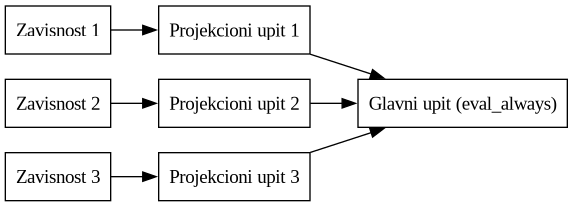
\includegraphics[width=4in, height=1.6in]{assets/images/projection_query.png}
\end{center}
\caption{Upotreba "eval\_always" modifikatora u projekcionom šablonu}
\label{lst:projection_query}
\end{listing}
\subsection{Tipizirana medju reprezentacija visokog nivoa - THIR (Typed HIR)}

Tipizirana medju reprezentacija HIR je posredna reprezentacija izvornog koda koja se generiše nakon provere tipova, jer je potrebno
da su tipovi unutar celog stabla popunjeni. THIR sadrži samo tela (obično tela funkcija) tj. izvršni kod.
Posledica ovoga jeste nedostatak reprezentacija struktura i osobina. 
Rust ima odliku da ukoliko se koristi neki vid provere šablona (\verb|pattern matching|) svaki tip unutar 
šablona mora biti pokriven \ref{lst:pattern_matching}. Proveru da li je svaki tip obradjen izvršava THIR.

\begin{listing}[H]
\begin{minted}{rust}
pub enum IpAddrKind {
    V4,
    V6,
}

fn main() {
    let x = IpAddrKind::V4;
    match x {
        IpAddrKind::V4 => println!("Ovo je IPv4 adresa."), 
        // Pokriven IpAddrKind::V4
        IpAddrKind::V6 => println!("Ovo je IPv6 adresa.") 
        // Pokriven IpAddrKind::V6
        // Da je postojao IpAddrKind::V7 Rust bi zahtevao 
        // da i ta varijanta bude obradjena.
    }
}
\end{minted}
\caption{Provera šablona}
\label{lst:pattern_matching}
\end{listing}

Za razliku od HIR-a koji je perzistiran tokom celokupnog izvršavanja kompajlera, THIR se odbacuje momenta
kada više nema upotrebnu vrednost. Pored toga što su svi tipovi čvorova prisutni, THIR se odlukuje dodatnim 
pojednostavljivanjem koda:
\begin{enumerate}
    \item Automatska referenciranja i dereferenciranja su eksplicitna.
    \item Pozivi metoda i opterećeni operatori su konvertovani u obične pozive funkcija. 
    \item Obim životnog veka je eksplicitan.
\end{enumerate}
% Izrazi, iskazi i \verb|match| ruke se čuvaju zasebno. 

Pojednostavljenje čini THIR podobnim za proveru nebezbednog koda jer fundamentalno poseduje manje opcija, 
nebezbedni pozivi metoda i nebezbedni pozivi funkcija imaju identičnu reprezentaciju. Ova provera 
iskazuje grešku ako je nebezbedna operacija korišćena van \verb|unsafe| opsega.

\todo{THIR je kratak sam po sebi ali moguće je detaljnije obraditi pattern matching}
\subsection{Medjureprezentacija srednjeg nivoa - MIR (Mid-Level Intermediate Representation)}

Koncept medjureprezentacije srednjeg nivoa nije postojao od samog nastanka kompajlera. Medjutim,
kako je kompajler postajao sve kompleksniji uvidela se potreba za reprezentacijom koja može da 
se upotrebi u kontekstu inkrementalne kompilacije, kao i potreba da ta medjureprezentacija lako manipuliše 
kontrolom toka. Kontrola toka je bila vezana za apstraktno sintaksno stablo što se pokazalo nedovoljno fleksibilno. 
Graf kontrole toka je pravi alat za ovaj posao jer je kontrola toka eksplicitna. Graf kontrole toka je 
struktuiran kao grupa osnovnih blokova koji su povezani granama. Ključna ideja bloka jeste da je to grupa naredbi (iskaza) 
koja se izvršava zajedno. Svaki put kada se granom dodje do novog bloka, sve naredbe tog bloka moraju da se izvrše, pa tek onda postoji mogućnost 
da se grana dalje. Poslednja nareba unutar bloka se naziva terminator. Brojni izrazi \ref{lst:block_code} koji se koriste u Rust jeziku se kompajliraju na 
više osnovnih blokova \ref{lst:block_block}.

\begin{listing}[H]
\begin{minted}{rust}
a = 1;
if some_variable {
    b = 1;
} else {
    c = 1;
}
d = 1;
\end{minted}
\caption{Isečak koda koji se prevodi u više osnovnih blokova}
\label{lst:block_code}
\end{listing}


\begin{listing}[H]
\begin{minted}{text}
BB0: {
    a = 1;
    if some_variable {
        goto BB1;
    } else {
        goto BB2;
    }
}
BB1: {
    b = 1;
    goto BB3;
}
BB2: {
    c = 1;
    goto BB3;
}
BB3: {
    d = 1;
    ...
}
\end{minted}
\caption{Isečak koda u formi osnovih blokova}
\label{lst:block_block}
\end{listing}

Stek (\verb|Stack|) je LIFO (\verb|Last in First Out|) struktura podataka koju kompajler koristi da skladišti argumente funkcija,
lokalne promenljive i privremene promenljive. U MIR reprezentaciji memorijske lokacije na steku su identifikovane pomoću indeksa. 
Indeks se označava celobrojnom vrednošću koju prethodi donja crta (npr. \verb|_1|, \verb|_2|). Indeks \verb|_0| je specijalan, u njemu
se skladišti povratna vrednost. Mesta su izrazi koji identifikuju lokaciju u memoriji. Mesto može biti sam indeks (\verb|_1|) ili može biti
projekcija (\verb|_1.polje|). Projekcije su polja ili druge konstrukcije koje proizilaze iz mesta. Pristup polju je projekcija, za \verb|_1.polje|, \verb|_1| je mesto dok je \verb|polje| projekcioni element.
Dereferenciranje je takođe projekcija, za \verb|*_1|, \verb|_1| je mesto dok je \verb|*| projekcioni element. 
Desne vrednosti (\verb|RValues|) su izrazi koji generišu vrednost. Zovu se desne vrednosti zato što 
stoje sa desne strane operatora dodele (\verb|=|). Operandi su argumenti desne vrednosti. Argument može biti konstanta ili mesto (kao što je \verb|_1|).

Strukturu srednje medjureprezentacije je najlakše razumeti prevodjenjem jednostavnih programa poput \ref{lst:snippet-before-mir}. U dodatku \ref{lst:unoptimized-mir} se nalazi neoptimizovana njegova srednja medjureprezentacija. Glavna razlika izmedju optimizovane i neoptimizovanje srednje medjureprezentacije jeste to što neoptimizovana medjureprezentacija sadrži eksplicitne iskaze \verb|StorageLive| i \verb|StorageDead| unutar osnovnih blokova. Iskaz \verb|StorageLive| pruža informaciju da je promenljiva navedena u iskazu živa tj.
da ju je moguće koristiti u daljem izvršavanju. Iskaz \verb|StorageDead| pruža informaciju da je promenljiva navedena u iskazu mrtva
tj. nije je više moguće koristiti. Samim time ovo se pokazuje kao pravo mesto da se sprovodi dealokacija memorije.
Jedina informacija koju srednja reprezentacija ne zna eksplicitno jeste da li se dogodio prenos vlasništva. Ovu informaciju dobija na osnovu tipa promenljive.

\begin{listing}[H]
\begin{minted}{text}
fn main() {
    let mut vec = Vec::new();
    vec.push(1);
    vec.push(2);
}
\end{minted}
\caption{Isečak koda koji se prevodi u MIR}
\label{lst:snippet-before-mir}
\end{listing}

MIR se generiše na osnovu \verb|mir_build| upita unutar THIR-a tj. sprovodi se samo nad izvršnim kodom. Upit se može uočiti u dodatku 3 \ref{lst:safety_check}.a Funkcije koje generišu MIR spadaju u jednu od dve grupe. Prva grupa su funkcije koje generišu naredbe.
Ove funkcije uzimaju osnovni blok kao argument i dodaju mu nove naredbe. Druga grupa su funkcije koje generišu nove osnovne 
blokove. Konstrukcija \verb|if| \verb|else| zahteva generisanje grafa oblika dijamanta tj. dva nova osnovna bloka.


Dokazati bezbednost formalno je izuzetno težak 
problem u bilo kojem Turing kompletnom jeziku. Naime, reprezentacija srednjeg nivoa se generiše da bude dovoljno jednostavna 
da bi se u jednom trenutku formalni dokazi mogli pisati na račun nje. 

Optimizacije specifične za Rust su teško izvodljive bez uvodjenja reprezentacije pre interakcije sa LLVM-om. Srednja medjureprezentacija 
ima mogućnost da sprovede analizu da li je bezbedno primeniti optimizaciju, i ako jeste da je unapred primeni. Uvodjenjem srednje medjureprezentacije bolje povlači granica izmedju samog jezika i LLVM-a jer 
semantika jezika nije vezana za konverziju u LLVM medjureprezentaciju.


Medjureprezentacija srednjeg nivoa nastaje procesuiranjem izraza iz \verb|THIR| reprezentacije rekurzivno.
U HIR-u optimizacija \verb|for| petlje je svedena na \verb|while(let)| u MIR-u se prevodi na \verb|loop match| 
primitivu \ref{lst:mir_for_1}.  Pozivi metoda su prevedeni u pozive funkcija još u THIR-u.

\begin{listing}[H]
\begin{minted}{rust}
let mut iterator = IntoIterator::into_iter(vec);
loop {
    match Iterator::next(&mut iterator){
        Some(elem) => process(elem),
        None => break,
    }
}
\end{minted}
\caption{"while let" posle pojednostavljenja}
\label{lst:mir_for_1}
\end{listing}

Reprezentacija srednjeg nivoa dozvoljava za još jedan vid optimizacije na nivou frontenda pojednostavljivanjem
sintakse na primitive koje nisu dostupne u regularnom jeziku.

\begin{listing}[H]
\begin{minted}{rust}
let mut iterator = IntoIterator::into_iter(vec);

loop:
    match Iterator::next(&mut iterator) {
        Some(elem) => { process(elem); goto loop; }
        None => { goto break; }
    }

break:
\end{minted}
\caption{"while let" posle pojednostavljenja}
\label{lst:mir_for_2}
\end{listing}

Izraz \verb|goto| je u inženjerskoj zajednici gledan sa visine jer kontrola toka nakon odredjene kompleksnosti
postaje nerazumljiva. Rust iz istog razloga ne dozvoljava upotrebu ove ključne reči, ali u MIR-u svodi 
petlju na najjednostavniji oblik \ref{lst:mir_for_2}.

\newpage
U isečku koda \ref{lst:mir_for_2}, jedina kompleksnija sintaktička celina je \verb|match|. U samom jeziku 
grupisanje provere i pristup podatku je smisleno ali u MIR-u se odvaja na dve celine \ref{lst:mir_for_3}.

\begin{listing}[H]
\begin{minted}{rust}
loop:
    let tmp = Iterator::next(&mut iterator);
    
    switch tmp {
        Some => {
            let elem = (tmp as Some).0;
            process(elem);
            goto loop;
        }
        None => {
            goto break;
        }
    }
    
break:
    ....
\end{minted}
\caption{"while let" posle pojednostavljenja}
\label{lst:mir_for_3}
\end{listing}

Naime ovako sveden kod nikada nije tekstualnom obliku. MIR je graf kontrole toka koji se može predstaviti
uz pomoć \verb|graphviz|-a \ref{lst:mir_print}. Filter mora biti zadatat prilikom poziva ove komande. 
Za prikaz celokupnog izlaza koristi se \verb|all| filter, dok ako je neka pojedinačna funkcija od interesovanja
njeno ime (mnogo češće slučaj).

\begin{listing}[H]
\begin{minted}{bash}
cargo rustc -- -Z dump-mir=[filter] -Z dump-mir-graphviz
\end{minted}
\caption{Ispis i prikaz MIR-a}
\label{lst:mir_print}
\end{listing}

\todo{MIR je opsežan, ne izgleda kao u primerima (umereni nivo obfuskacije). Ovde ima još značajno puno sadržaja koji nije opisan.}

\section{Zaključak}
\section{Literatura}

\begin{thebibliography}
    \raggedright
\bibitem{msrc} 
    MSRC, “A proactive approach to more secure code | MSRC Blog | 
    Microsoft Security Response Center,” Microsoft.com, Jul. 16, 2019. 
    \url{https://msrc.microsoft.com/blog/2019/07/a-proactive-approach-to-more-secure-code/} 
    (pristupljeno Sep. 08, 2024).

    \bibitem{parsing} 
    “Parsing” Rochester.edu, 2024.
    \url{https://www.cs.rochester.edu/u/nelson/courses/csc_173/grammars/parsing.html#:~:text=Recursive%2Ddescent%20parsing%20is%20one,non%2Dterminal%20with%20a%20procedure} 
    (pristupljeno Sep. 21, 2024).

    \bibitem{dragonbook} 
    A. V. Aho, M. S. Lam, R. Sethi, and J. D. Ullman, \emph{Compilers: Principles, Techniques, and Tools}, 2nd ed. Boston, MA, USA: Addison-Wesley, 2006.

    \bibitem{rust-guide} 
    “Getting Started - Rust Compiler Development Guide,” Rust-lang.org, 2024. 
    \url{https://rustc-dev-guide.rust-lang.org/getting-started.html} (pristupljeno Sep. 28, 2024).

    \bibitem{rust-reference}
    “Introduction - The Rust Reference,” Rust-lang.org, 2015. 
    \url{https://doc.rust-lang.org/reference/introduction.html} (pristupljeno Sep. 29, 2024).
    
    \bibitem{rustonomicon}
    “Meet Safe and Unsafe - The Rustonomicon,” Rust-lang.org, 2024. 
    \url{https://doc.rust-lang.org/nomicon/meet-safe-and-unsafe.html} (pristupljeno Sep. 29, 2024).

    \bibitem{editions}
    “What are editions? - The Rust Edition Guide,” Rust-lang.org, 2024.
    \url{https://doc.rust-lang.org/edition-guide/editions/} (pristupljeno Okt. 03, 2024).

    \bibitem{unstable}
    “The Unstable Book - The Rust Unstable Book,” Rust-lang.org, 2024. 
    \url{https://doc.rust-lang.org/unstable-book/index.html} (pristupljeno Okt. 06, 2024).

    \bibitem{unstable-flagsunstable}
    Li, Chenghao, et al. “Demystifying Compiler Unstable Feature Usage and Impacts in the Rust Ecosystem.” 26 Oct. 2023. arXiv, Pristupljeno 6 Oct. 2024. 

    \bibitem{rust-language}
    Bugden W, Alahmar A. Rust: The programming language for safety and performance. arXiv preprint arXiv:2206.05503. 2022 Jun 11.

    \bibitem{supply-chain}
    P. Mainardi, “The Rising Threat of Software Supply Chain Attacks: Managing Dependencies of Open Source projects,” Linuxfoundation.eu, Aug. 15, 2023.
    \url{https://linuxfoundation.eu/newsroom/the-rising-threat-of-software-supply-chain-attacks-managing-dependencies-of-open-source-projects} (pristupljeno Okt. 20, 2024).

    \bibitem{oss-architecture}
    “The Architecture of Open Source Applications (Volume 1)LLVM,” Aosabook.org, 2024. 
    \url{https://aosabook.org/en/v1/llvm.html} (pristupljeno Nov. 04, 2024).

    \bibitem{llvm}
    “The LLVM Compiler Infrastructure Project,” Llvm.org, 2024. 
    \url{https://llvm.org/} (pristupljeno Nov. 04, 2024).
\end{thebibliography}
\section{Dodatak 1}

\begin{listing}[H]
\begin{minted}{rust}
#[proc_macro_attribute]
pub fn expand_body(_attr: TokenStream, _item: TokenStream) -> TokenStream {
    let fun = format!("fn missing_body() 
    {{ println!(\"I'm not missing body anymore.\"); }}");

    let stream: TokenStream = fun.parse().unwrap();

    stream
}

#[expand_body]
fn missing_body();

fn main() {
    missing_body();
}
\end{minted}
\caption{Dodavanje tela funkcije uz pomoć makroa}
\label{lst:bonus_body_expand}
\end{listing}



\section{Dodatak 2}
\begin{figure}[H]
\begin{listing}[H]
\begin{minted}{rust}
fn try_mark_green(tcx, current_node) -> bool {
// Fetch the inputs to `current_node`, i.e. get the nodes that the direct
// edges from `node` lead to.
let dependencies = tcx.dep_graph.get_dependencies_of(current_node);
// Now check all the inputs for changes
for dependency in dependencies {
match tcx.dep_graph.get_node_color(dependency) {
Green => {
// This input has already been checked before and it has not
// changed; so we can go on to check the next one
}
Red => {
// We found an input that has changed. We cannot mark
// `current_node` as green without re-running the corresponding query.
    return false
}
Unknown => {
// This is the first time we look at this node. Let's try
// to mark it green by calling try_mark_green() recursively.
    if try_mark_green(tcx, dependency) {
// We successfully marked the input as green, on to the next.
    } else {
// We could *not* mark the input as green. This means we
// don't know if its value has changed. In order to find
// out, we re-run the corresponding query now!
        tcx.run_query_for(dependency);
// Fetch and check the node color again. Running the query
// has forced it to either red (if it yielded a different
// result than we have in the cache) or green (if it
// yielded the same result).
        match tcx.dep_graph.get_node_color(dependency) {
            Red => {
// The input turned out to be red, so we cannot mark `current_node` as green.
                return false
            }
            Green => {
// Re-running the query paid off! The result is the same as before, 
// so this particular input does not invalidate `current_node`.
            }
            Unknown => {
// There is no way a node has no color after re-running the query.
                panic!("unreachable") } } } } } }
tcx.dep_graph.mark_green(current_node);
true }
\end{minted}
\caption{Implementacija algoritma "try-mark-green"}
\label{lst:bonus_try_mark_green}
\end{listing}
\end{figure}
\section{Podaci o kandidatu}


Kandidat Aleksa Bajat rođen je 2001. godine u Novom Sadu. Završio je prirodno-matematički smer na engleskom jeziku 
u gimnaziji "Jovan Jovanović Zmaj" 2019. godine. Tokom sve četiri godine gimnazije uspešno je pohadjao 
"Centar za mlade talente" kompanije Schneider Electric.  Godine 2019. upisao je Fakultet 
Tehničkih Nauka u Novom Sadu, gde je ispunio sve obaveze i položio sve ispite predviđene 
studijskim programom sa prosečnom ocenom 9.03.

\end{document}
